\documentclass[14pt,aspectratio=169]{beamer}

\usepackage[utf8]{inputenc}
\usepackage{amsmath, amssymb, amsfonts, cancel}
\usefonttheme[onlymath]{serif}
\usetheme{Warsaw}
\setbeamertemplate{navigation symbols}{}
\setbeamertemplate{headline}{}
\setbeamercovered{transparent}
\mode<presentation>

\begin{document}

\title{Session 3 : Circles}
\subtitle{\textit{Precalculus: A Problem-Solving Approach}}
\author{JING ARQUERO}
\institute{{\normalsize University of the East - Manila} \\ {\normalsize C.M. Recto Ave., Manila, Philippines}}
\date{All Rights Reserved {\textrm{\copyright}} 2019}

\begin{frame}
 \maketitle
\end{frame}

\begin{frame}{Session Outline}
    \begin{enumerate}
     \item The Cartesian Plane
     \item Definition of a Point
     \item Distance between Two Points
     \item The Circle
     \item References
    \end{enumerate}

\end{frame}

\begin{frame}{The Cartesian Plane}
  \begin{columns}
   \column{0.4\textwidth}\centering
    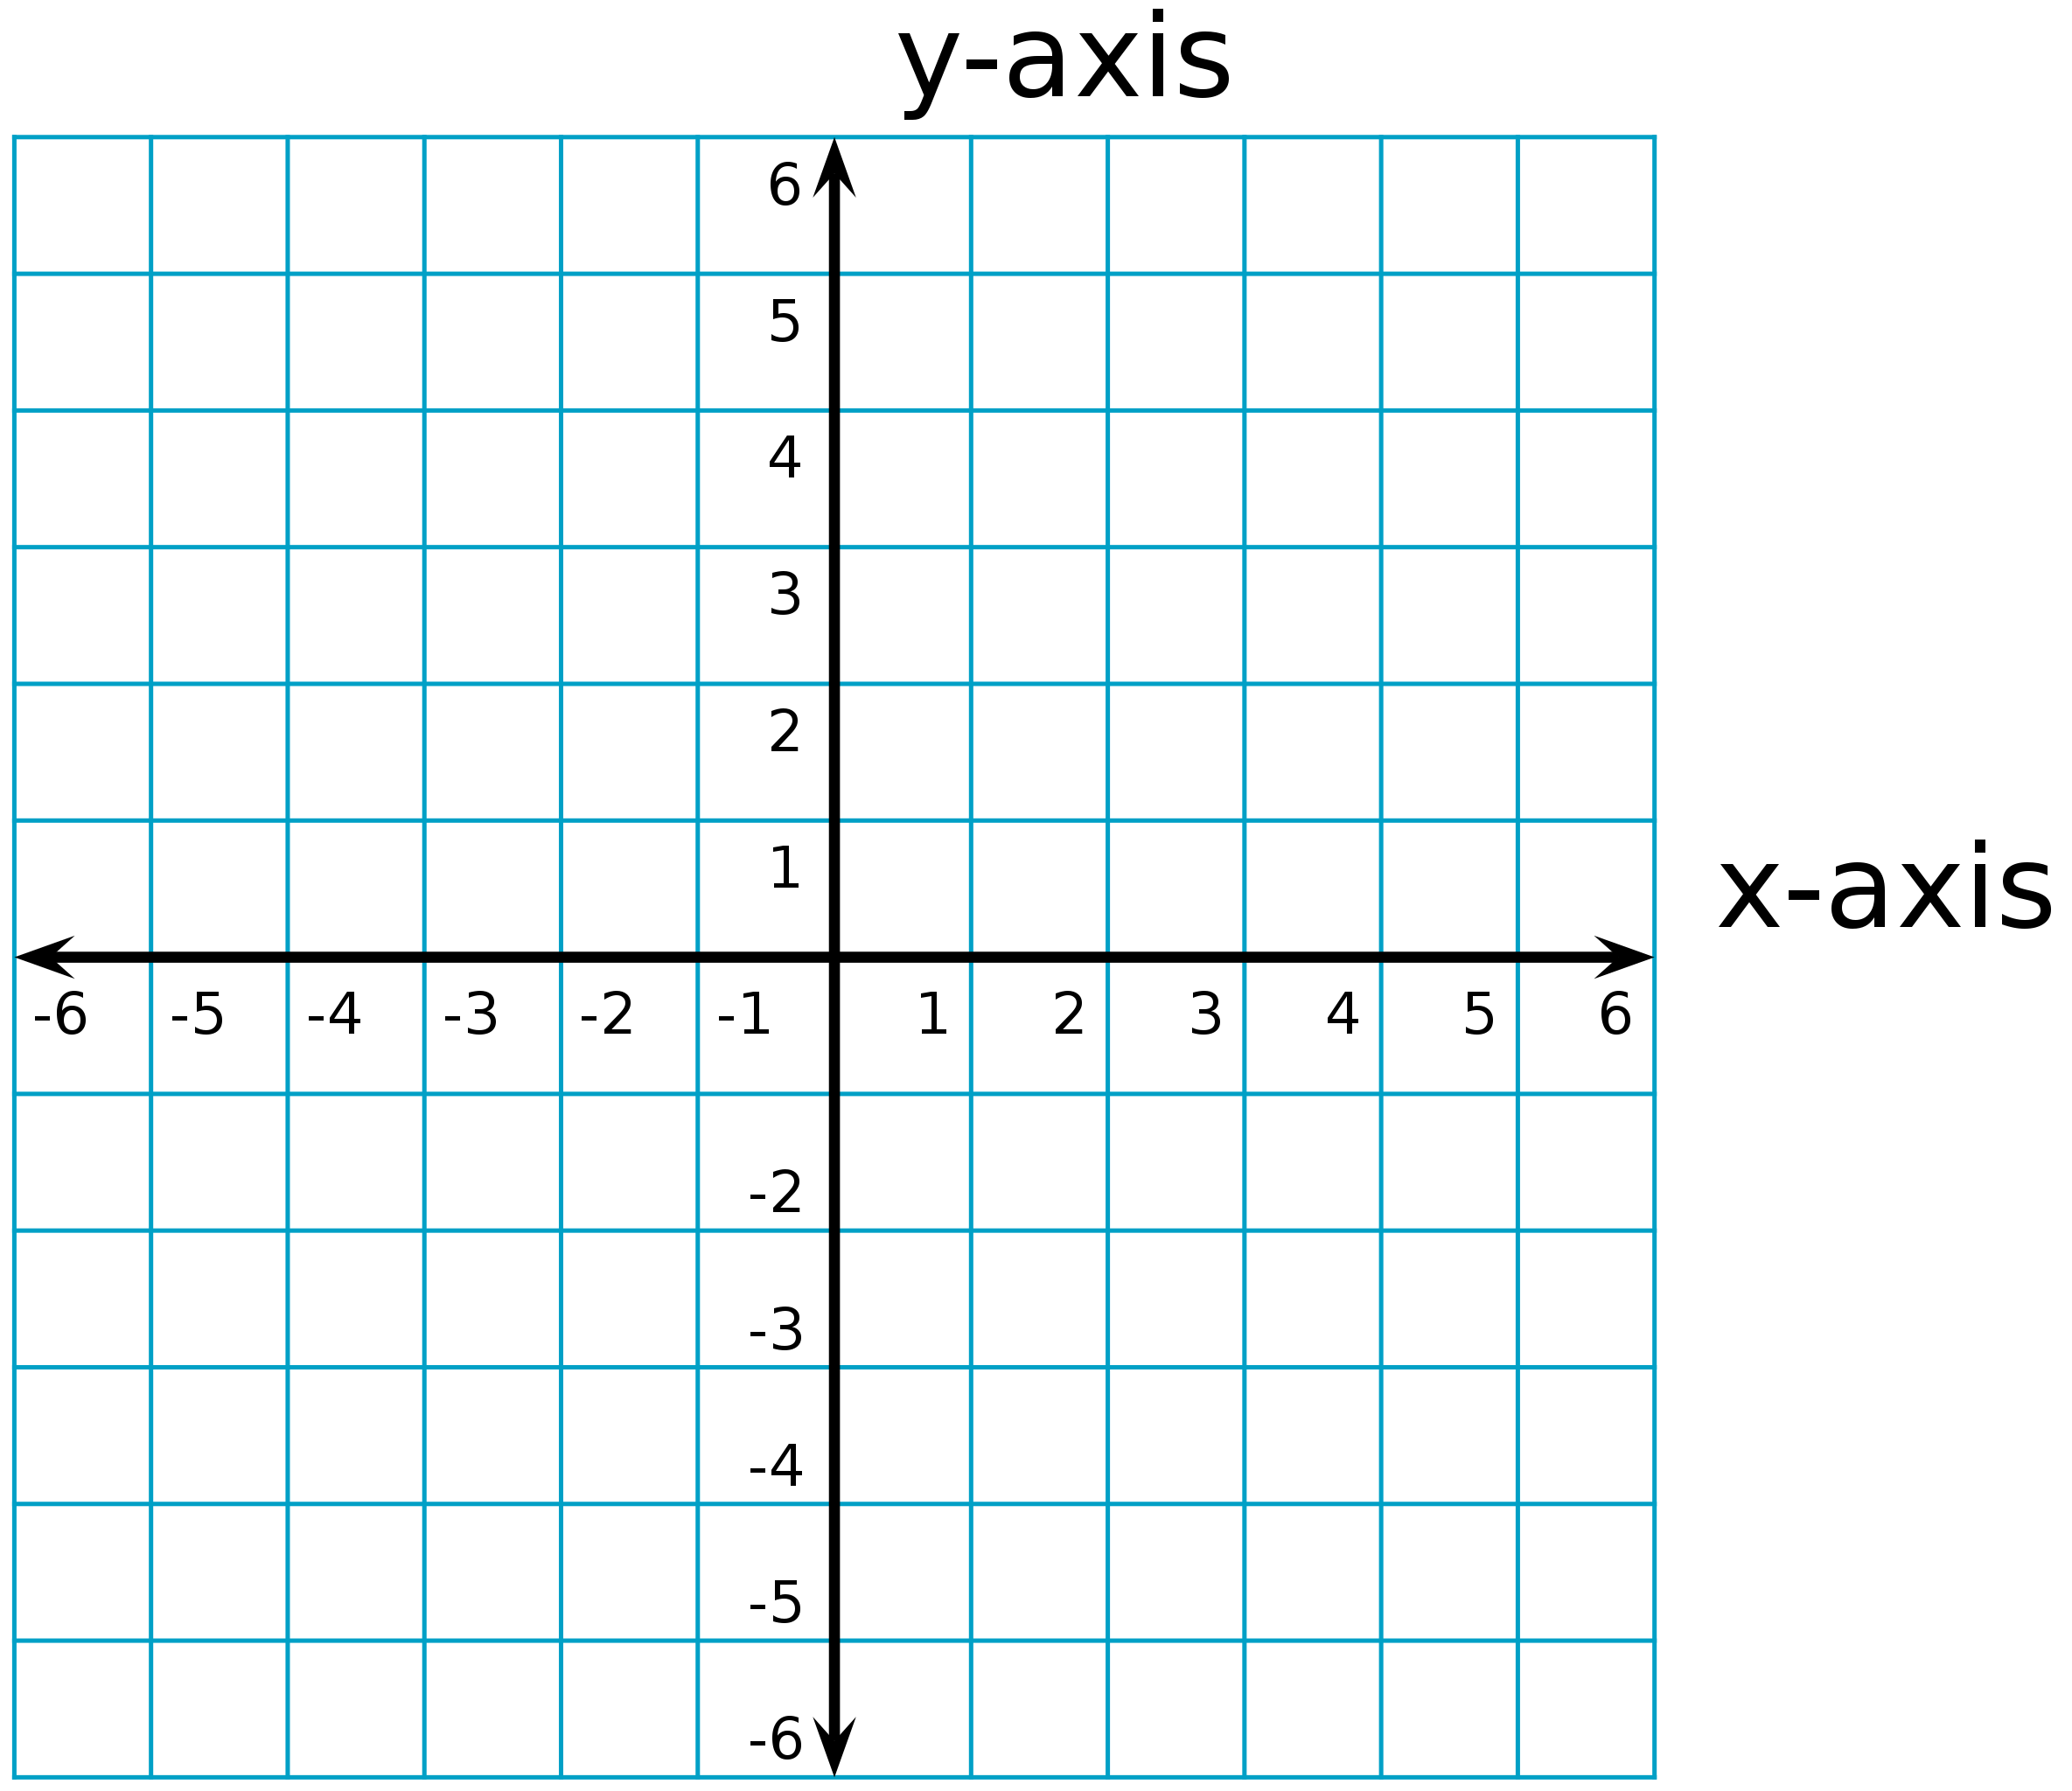
\includegraphics[width=1\textwidth]{image01}\\The Rectangular Coordinate System
   \column{0.6\textwidth}
    \begin{block}{Parts of a Plane}
     \begin{itemize}
      \item $x-axis$, $x-values$
      \item $x-values$ moves right to $+\infty$
      \item $x-values$ moves left to $-\infty$
      \item $y-axis$, $y-values$
      \item $y-values$ shifts up to $+\infty$
      \item $y-values$ shifts down to $+\infty$
      \item $x-axis\perp y-axis$ at $O(0,0)$
      \item Units $n$ and Gridlines
     \end{itemize}

    \end{block}

  \end{columns}

\end{frame}

\begin{frame}{The Four Quadrants}
  \begin{columns}
   \column{0.4\textwidth}\centering
    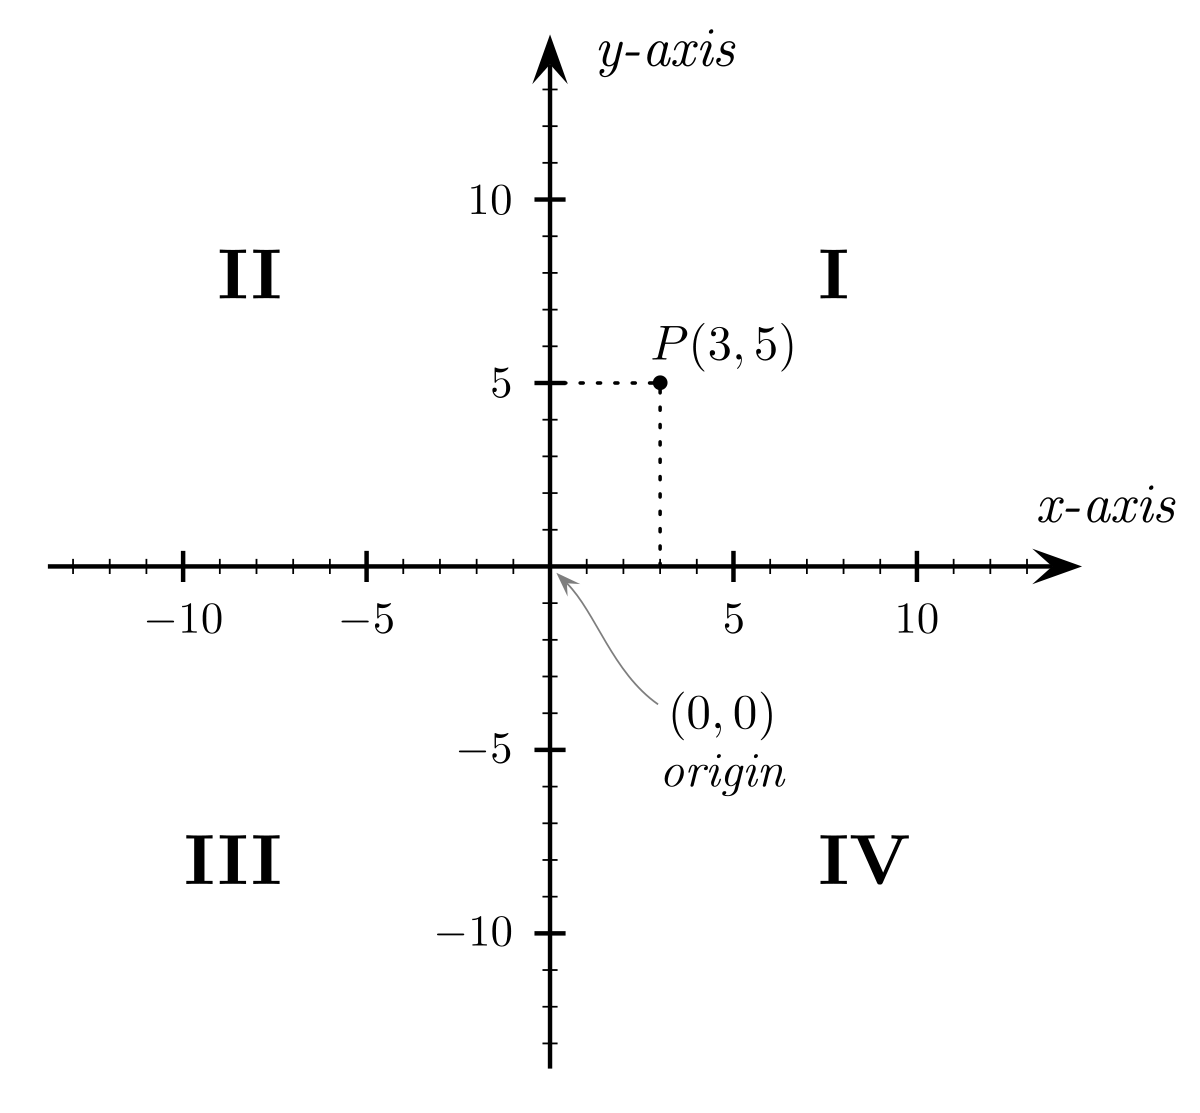
\includegraphics[width=1\textwidth]{image02}\\The Quadrants
   \column{0.6\textwidth}
    \begin{block}{Values in the Quadrants}
     \begin{itemize}
      \item First Quadrant $I(+x,+y)$
      \item Second Quadrant $II(-x,+y)$
      \item Third Quadrant $III(-x,-y)$
      \item Fourth Quadrant $IV(+x,-y)$

     \end{itemize}

    \end{block}

    \begin{exampleblock}{Realizations}
     An infinite plane can be divided into smaller but infinite planes.
    \end{exampleblock}


  \end{columns}

\end{frame}

\begin{frame}{The Definition of a Point}
  \begin{columns}
   \column{0.4\textwidth}\centering
    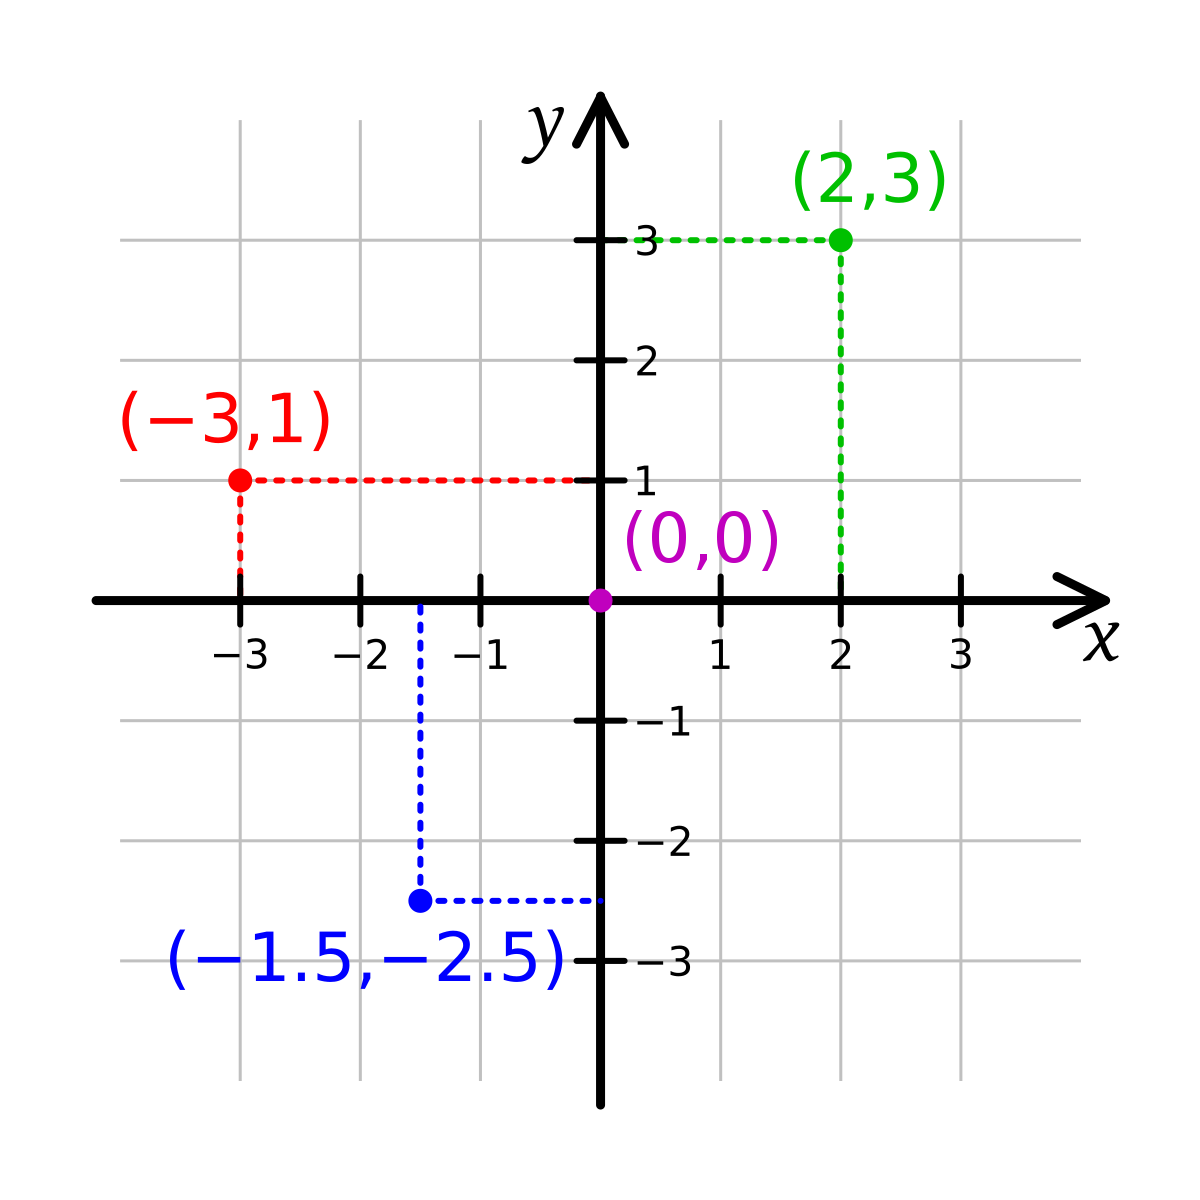
\includegraphics[width=1\textwidth]{image03}\\Some Points on the Plane
   \column{0.6\textwidth}
    \begin{block}{Points}
     \begin{itemize}
      \item Point $P(x,y)$ is an exact two-dimensional location
      \item $P$, Point Name
      \item $x$, $x-value$ or abscissa
      \item $y$, $y-value$ or ordinate
      \item $(x,y)$, \textit{ordered pair} or coordinates
      \item $\bullet$ Point, Close Point
      \item $\circ$ Hollow Point, Open Point
      \item Locations can be estimated

     \end{itemize}

    \end{block}


  \end{columns}

\end{frame}

\begin{frame}{Problems 3.1 - 3.8}
 \begin{exampleblock}{Estimate the Location of the following Points}
  \begin{enumerate}
   \item $A(1,2)$
   \item $B(5,0)$
   \item $C(-3,4)$
   \item $D(0,4)$
   \item $E(7,-3)$
   \item $F(-4,0)$
   \item $G(-\pi,-\sqrt{2})$
   \item $H(0, -\pi)$
  \end{enumerate}

 \end{exampleblock}

\end{frame}


\begin{frame}{Domain \& Range}
  \begin{columns}
   \column{0.4\textwidth}\centering
    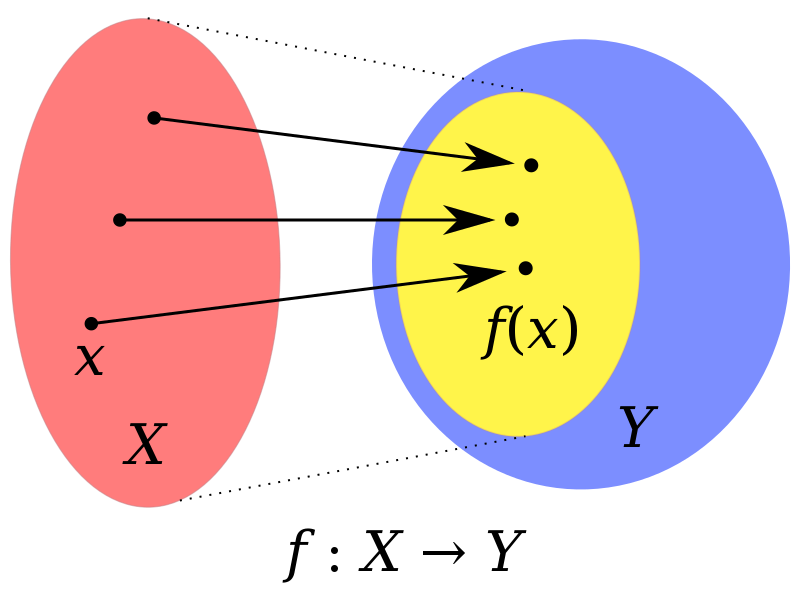
\includegraphics[width=1\textwidth]{image04}\\Mapping Diagram
   \column{0.6\textwidth}
    \begin{block}{Domain $x$ and Range $y$} \centering
      \begin{itemize}
       \item Two Points make a line (Euclid)
       \item Domain, set of all $x-values$
       \item Range, set of all $y-values$
      \end{itemize}
    \end{block}

    \begin{block}{Interval Notation}
     \begin{itemize}
      \item Exclusivity $(x), >, <, \neq, \circ$
      \item Inclusivity $[x], \geq, \leq, =, \bullet$
      \item Infinity ($\pm\infty$) is always exclusive
     \end{itemize}

    \end{block}

  \end{columns}

\end{frame}

\begin{frame}{Problems 3.9 - 3.16}
 \begin{exampleblock}{Illustrate reference lines using the following notations}
  \begin{enumerate}
   \item $x(-\infty, +\infty)$
   \item $x(-\infty, 8)$
   \item $x(-\infty, 6]$
   \item $x(11, +\infty)$
   \item $x[-2,+\infty)$
   \item $x[4, 10] \cup (11,18)$
   \item $x(6, 12]\cup [18,22)$
   \item $x[-1, 9]\cup (15,27]$
  \end{enumerate}

 \end{exampleblock}

\end{frame}

\begin{frame}{Distance Between Two Points}
  \begin{columns}
   \column{0.4\textwidth}\centering
    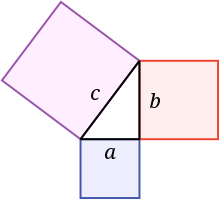
\includegraphics[width=1\textwidth]{image05}\\The Pythagorean Theorem
   \column{0.6\textwidth}
    \begin{block}{Increment $\Delta$} \centering
      $\Delta P = P_1 - P_2$ \\
      Also, \textit{discriminant} $\Delta=b^2-4ac$
    \end{block}

    \begin{block}{Pythagorean Theorem} \centering
     $a^2 + b^2 = c^2$
    \end{block}

    \begin{block}{Distance $d$}\centering
    $d=\sqrt{\Delta x^2 + \Delta y^2}$
    \end{block}

  \end{columns}

\end{frame}

\begin{frame}{The Circle}
 \begin{columns}
  \column{0.4\textwidth}\centering
  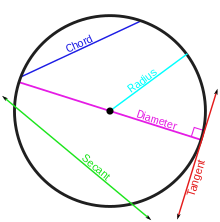
\includegraphics[width=1\textwidth]{image06}\\Circle \& Its Parts
  \column{0.6\textwidth}
    \begin{block}{Definition of a Circle}
      \begin{itemize}
       \item A conic section produced when a double-napped cone is sliced by a plane parallel to the base
       \item A circle is the set of all points $P_n$ having the same distance from a center point $C(h,k)$
      \end{itemize}
    \end{block}
      \begin{block}{The Radius}
      The Radius $r$ is the distance from the center of a circle to a point on the circle.

    \end{block}

 \end{columns}

\end{frame}

\begin{frame}{Problems 3.17 - 3.24}

 \begin{exampleblock}{Find the Standard and General Equations, and estimate the graphs of the following circles.}
  \begin{enumerate}
   \item Center at the $origin$, radius 4
   \item Center $(-4,3)$, radius $\sqrt{7}$
   \item $A(3,1), \; r=5$
   \item $B(-2,-1), \; r=4$
   \item $C(3,2), \; r=3$
   \item Center $(5,-6)$, tangent to the $y-axis$
   \item Center $(5,-6)$, tangent to the $x-axis$
   \item Has a diameter with endpoints $A(-1,4), B(4,2)$

  \end{enumerate}

 \end{exampleblock}

\end{frame}

\begin{frame}{The Equation of a Circle}
  \begin{columns}
   \column{0.4\textwidth}\centering
   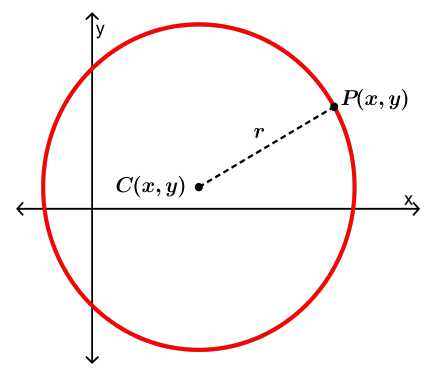
\includegraphics[width=1\textwidth]{image07}\\The Radius
   \column{0.6\textwidth}
    \begin{block}{The Radius}\centering
     $d\to r=\sqrt{\Delta x^2 +\Delta y^2}$
    \end{block}

    \begin{block}{General Equation of a Circle} \centering
     $Ax^2 + By^2 + Cx + Dy + E = 0$\\
     Condition: $A,B > 0$
    \end{block}

    \begin{block}{Standard Equation of a Circle} \centering
     $(x-h)^2 + (y-k)^2 = r^2$ \\
     $h,k$ are vertices of circle $C$

    \end{block}



  \end{columns}

\end{frame}

\begin{frame}{Problems 3.25 - 3.32}
 \begin{exampleblock}{Find the radius $r$}
  \begin{enumerate}
   \item $A(0,0),   \;S(0,3)$
   \item $B(1,-7),    \;T(4,-7)$
   \item $C(-2,-6),   \;U(-8,11)$
   \item $D(-3,5),  \;V(-12,-15)$
   \item $E(-4,4),   \;W(-14,-13)$
   \item $F(-5,-3),  \;X(-10,9)$
   \item $G(6,-2),  \;Y(6,-5)$
   \item $H(7,1),  \;Z(2,1)$
  \end{enumerate}

 \end{exampleblock}

\end{frame}

\begin{frame}{The Perfect Square}
 \begin{columns}
  \column{0.4\textwidth}\centering
  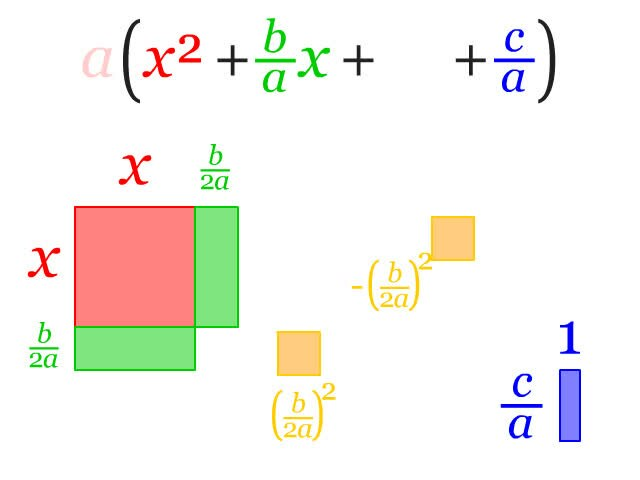
\includegraphics[width=1\textwidth]{image08}\\Completing Squares
  \column{0.6\textwidth}
  \begin{block}{The Perfect Square}\centering
   $x\times x = x^2$ \\
   $(x\pm y)^2 = x^2 \pm 2xy + y^2$ \\
   $PST: ax^2 + bx + c$
  \end{block}

  \begin{block}{Missing Middle Term}\centering
   Given $ax^2 + c$
   then $bx = 2\sqrt{ax^2}\sqrt{c}$
  \end{block}

  \begin{block}{Missing Final Term}\centering
   Given $ax^2 + bx$
   then $c=\left(\frac{bx}{2\sqrt{ax^2}}\right)$
  \end{block}


 \end{columns}

\end{frame}

\begin{frame}{Problems 3.33 - 3.40}
 \begin{exampleblock}{Complete the following squared equations, and find the values of $x$}
  \begin{enumerate}
   \item $x^2 - 1 = 0$
   \item $y^2 + 4 = 0$
   \item $x^2 - 6x - 4 = 0$
   \item $y^2 - 14x + 1= 0$
   \item $16x^2 + 96x = 45$
   \item $4y^2 - 32y = 12$
   \item $x^2 + 2x = -1$
   \item $2x^2 + 3x = 7$
  \end{enumerate}

 \end{exampleblock}

\end{frame}


\begin{frame}{Problems 3.41 - 3.48}
 \begin{exampleblock}{Transform the following General Equations into Standard Equations, and find the radius $r$}
  \begin{enumerate}
   \item $x^2 + y^2 - 6x = 7$
   \item $x^2 + y^2 -14x + 2y = -14$
   \item $16x^2 + 16y^2 + 96x-40y=315$
   \item $x^2 +y^2 -5x +4y = 96$
   \item $4x^2 + 4y^2 + 40x - 32y = 5$
   \item $x^2 + y^2 - 4x + 6y + 4 = 0$
   \item $x^2 + y^2 - 8x -16y-89=0$
   \item $x^2 + y^2 + 1 = 0$
  \end{enumerate}

 \end{exampleblock}

\end{frame}

\begin{frame}{Seatwork}
\textbf{GENERAL DIRECTIONS:}
\begin{itemize}
 \item Only write with a black-inked ballpoint pen
 \item Read the instructions and problems carefully
 \item Legibly write your solutions, and box your final answers
 \item Avoid cheating, using devices, and making erasures
 \item Physical Scientific Calculators are allowed
\end{itemize}

 \begin{block}{IT'S YOUR TURN}
    Answer \emph{pg. 17} Nos. 1 - 2
 \end{block}

 \begin{block}{IT'S YOUR TURN}
  Answer \emph{pg. 19} Nos. 1 - 3
 \end{block}


\end{frame}







\begin{frame}{References}
\textbf{DOCUMENTATION}\\
 This slide presentation is made with {\textrm \LaTeX}.
 The source code is available at:
 \texttt{https://github.com/redundies/ueshsprecal}\\~\\

 \textbf{REFERENCES}
 \begin{itemize}
  \item Garces, Ian June et. al (2016) \textit{Precalculus: Specialized Subject}
  \item Tamayo, Joycelyn et. al (2018) \textit{Precalculus for SHS Students}
  \item De Guzman, Danilo et. al (2019) \textit{Precalculus: A Worktext}
  \item Most Images from (\texttt{https://wikimedia.com}), {\sc PD-CC0L}
 \end{itemize}


\end{frame}
\end{document}
